%% For double-blind review submission, w/o CCS and ACM Reference (max submission space)
\documentclass[sigplan,screen]{acmart}\settopmatter{printfolios=true,printccs=false,printacmref=false}
%% For double-blind review submission, w/ CCS and ACM Reference
%\documentclass[sigplan,review,anonymous]{acmart}\settopmatter{printfolios=true}
%% For single-blind review submission, w/o CCS and ACM Reference (max submission space)
%\documentclass[sigplan,review]{acmart}\settopmatter{printfolios=true,printccs=false,printacmref=false}
%% For single-blind review submission, w/ CCS and ACM Reference
%\documentclass[sigplan,review]{acmart}\settopmatter{printfolios=true}
%% For final camera-ready submission, w/ required CCS and ACM Reference
%\documentclass[sigplan]{acmart}\settopmatter{}


%% Conference information
%% Supplied to authors by publisher for camera-ready submission;
%% use defaults for review submission.
\acmConference[ICFP'19]{ACM SIGPLAN International Conference on Functional Programming}{August 18--23, 2019}{Berlin, Germany}
\acmYear{2019}
\acmISBN{} % \acmISBN{978-x-xxxx-xxxx-x/YY/MM}
\acmDOI{} % \acmDOI{10.1145/nnnnnnn.nnnnnnn}
\startPage{1}

%% Copyright information
%% Supplied to authors (based on authors' rights management selection;
%% see authors.acm.org) by publisher for camera-ready submission;
%% use 'none' for review submission.
\setcopyright{none}
%\setcopyright{acmcopyright}
%\setcopyright{acmlicensed}
%\setcopyright{rightsretained}
%\copyrightyear{2018}           %% If different from \acmYear

%% Bibliography style
\bibliographystyle{ACM-Reference-Format}
%% Citation style
%\citestyle{acmauthoryear}  %% For author/year citations
%\citestyle{acmnumeric}     %% For numeric citations
%\setcitestyle{nosort}      %% With 'acmnumeric', to disable automatic
                            %% sorting of references within a single citation;
                            %% e.g., \cite{Smith99,Carpenter05,Baker12}
                            %% rendered as [14,5,2] rather than [2,5,14].
%\setcitesyle{nocompress}   %% With 'acmnumeric', to disable automatic
                            %% compression of sequential references within a
                            %% single citation;
                            %% e.g., \cite{Baker12,Baker14,Baker16}
                            %% rendered as [2,3,4] rather than [2-4].


%%%%%%%%%%%%%%%%%%%%%%%%%%%%%%%%%%%%%%%%%%%%%%%%%%%%%%%%%%%%%%%%%%%%%%
%% Note: Authors migrating a paper from traditional SIGPLAN
%% proceedings format to PACMPL format must update the
%% '\documentclass' and topmatter commands above; see
%% 'acmart-pacmpl-template.tex'.
%%%%%%%%%%%%%%%%%%%%%%%%%%%%%%%%%%%%%%%%%%%%%%%%%%%%%%%%%%%%%%%%%%%%%%


%% Some recommended packages.
\usepackage{booktabs}   %% For formal tables:
                        %% http://ctan.org/pkg/booktabs
\usepackage{subcaption} %% For complex figures with subfigures/subcaptions
                        %% http://ctan.org/pkg/subcaption

\usepackage{listings}
\lstset{
  % language=haskell%
       % , columns=flexible%
       , basewidth={0.6em, 0.5em},%
  frame=none,
  xleftmargin=2pt,
  stepnumber=1,
  numbers=left,
  numbersep=5pt,
  numberstyle=\ttfamily\tiny\color[gray]{0.3},
  belowcaptionskip=\bigskipamount,
  captionpos=b,
  escapeinside={*'}{'*},
  language=haskell,
  tabsize=2,
  emphstyle={\bf},
  commentstyle=\it,
  stringstyle=\mdseries\ttfamily,
  showspaces=false,
  % keywordstyle=\bfseries\sffamily,
  keywordstyle=\bfseries\ttfamily,
  columns=flexible,
  % basicstyle=\small\rmfamily,
  basicstyle=\small\ttfamily ,
  showstringspaces=false,
  morecomment=[l]\%,
  }

\ifxetex
\usepackage{fontspec}
\setmonofont[Scale=.8]{DejaVu Sans Mono}
\else
\usepackage{inconsolata}
\fi

\theoremstyle{acmplain}
\newtheorem{theorem}{Theorem}[section]
\theoremstyle{acmdefinition}
\newtheorem{remark}[theorem]{Remark}

\usepackage[obeyFinal]{todonotes}


%%% The following is specific to FHPNC '19 and the paper
%%% 'Lazy Evaluation in Infinite-Dimensional Function Spaces with Wavelet Basis'
%%% by Olivier Verdier and Justus Sagemüller.
%%%
\setcopyright{acmcopyright}
\acmPrice{15.00}
\acmDOI{10.1145/3331553.3342615}
\acmYear{2019}
\copyrightyear{2019}
\acmISBN{978-1-4503-6814-8/19/08}
\acmConference[FHPNC '19]{Proceedings of the 8th ACM SIGPLAN International Workshop on Functional High-Performance and Numerical Computing}{August 18, 2019}{Berlin, Germany}
\acmBooktitle{Proceedings of the 8th ACM SIGPLAN International Workshop on Functional High-Performance and Numerical Computing (FHPNC '19), August 18, 2019, Berlin, Germany}

\begin{document}

%% Title information
\title[Lazy Infinite Wavelet Expansion]
      {Lazy Evaluation in Infinite-Dimensional Function Spaces with Wavelet Basis}


\author{Justus Sagemüller}
\orcid{0000-0003-1882-1096}
\affiliation{
  \department{Faculty of Engineering and Science}
  \institution{Western Norway University of Applied Science}
  \streetaddress{Inndalsveien 28}
  \city{Bergen}
  \postcode{5020}
  \country{Norway}
}
\email{jsag@hvl.no}

%% Author with two affiliations and emails.
\author{Olivier Verdier}
\orcid{0000-0003-3699-6244}             %% \orcid is optional
\affiliation{
  \department{Faculty of Engineering and Science}
  \institution{Western Norway University of Applied Science}
  \streetaddress{Inndalsveien 28}
  \city{Bergen}
  % \state{Hordaland}
  % \postcode{5020}
  \country{Norway}
}
\email{olivier.verdier@hvl.no}
\affiliation{
  \department{Department of Mathematics}
  \institution{KTH-Royal Institute of Technology}
  % \streetaddress{Inndalsveien 28}
  \city{Stockholm}
  % \state{Hordaland}
  % \postcode{5020}
  \country{Sweden}
}
\email{olivierv@kth.se}


%% Abstract
%% Note: \begin{abstract}...\end{abstract} environment must come
%% before \maketitle command
\begin{abstract}
Vectors in numerical computation, i.e., arrays of numbers, often represent continuous functions.
We would like to reflect this with \emph{types}.
One apparent obstacle is that spaces of functions are typically infinite-dimensional,
while the code must run in finite time and memory.

We argue that this can be overcome: even in an infinite-dimensional space, the vectors \emph{can} in practice be stored in finite memory.
However, \emph{dual vectors} (corresponding essentially to \emph{distributions}) require infinite data structure.
The distinction is usually lost in the finite dimensional case, since dual vectors are often simply represented as vectors (by implicitly choosing a scalar product establishing the correspondence).
However, we shall see that an explicit type-level distinction between functions and distributions makes sense and allows directly expressing useful concepts such as the Dirac distribution, which are problematic in the standard finite-resolution picture.

The example implementation uses a very simple local basis that corresponds to a Haar Wavelet transform.
\end{abstract}


%% 2012 ACM Computing Classification System (CSS) concepts
%% Generate at 'http://dl.acm.org/ccs/ccs.cfm'.
\begin{CCSXML}
<ccs2012>
<concept>
<concept_id>10002950.10003714.10003736.10003737</concept_id>
<concept_desc>Mathematics of computing~Approximation</concept_desc>
<concept_significance>500</concept_significance>
</concept>
<concept>
<concept_id>10002950.10003648.10003703</concept_id>
<concept_desc>Mathematics of computing~Distribution functions</concept_desc>
<concept_significance>300</concept_significance>
</concept>
<concept>
<concept_id>10002950.10003714.10003715.10003726</concept_id>
<concept_desc>Mathematics of computing~Arbitrary-precision arithmetic</concept_desc>
<concept_significance>300</concept_significance>
</concept>
<concept>
<concept_id>10002950.10003714.10003715.10003750</concept_id>
<concept_desc>Mathematics of computing~Discretization</concept_desc>
<concept_significance>300</concept_significance>
</concept>
<concept>
<concept_id>10002950.10003741.10003746</concept_id>
<concept_desc>Mathematics of computing~Continuous functions</concept_desc>
<concept_significance>300</concept_significance>
</concept>
<concept>
<concept_id>10002950.10003712.10003713</concept_id>
<concept_desc>Mathematics of computing~Coding theory</concept_desc>
<concept_significance>100</concept_significance>
</concept>
<concept>
<concept_id>10002950.10003714.10003738</concept_id>
<concept_desc>Mathematics of computing~Integral equations</concept_desc>
<concept_significance>100</concept_significance>
</concept>
<concept>
<concept_id>10010147.10010148.10010164.10010166</concept_id>
<concept_desc>Computing methodologies~Representation of mathematical functions</concept_desc>
<concept_significance>500</concept_significance>
</concept>
<concept>
<concept_id>10010147.10010371.10010395</concept_id>
<concept_desc>Computing methodologies~Image compression</concept_desc>
<concept_significance>100</concept_significance>
</concept>
<concept>
<concept_id>10010405.10010432.10010442</concept_id>
<concept_desc>Applied computing~Mathematics and statistics</concept_desc>
<concept_significance>300</concept_significance>
</concept>
</ccs2012>
\end{CCSXML}

\ccsdesc[500]{Mathematics of computing~Approximation}
\ccsdesc[300]{Mathematics of computing~Distribution functions}
\ccsdesc[300]{Mathematics of computing~Arbitrary-precision arithmetic}
\ccsdesc[300]{Mathematics of computing~Discretization}
\ccsdesc[300]{Mathematics of computing~Continuous functions}
\ccsdesc[100]{Mathematics of computing~Coding theory}
\ccsdesc[100]{Mathematics of computing~Integral equations}
\ccsdesc[500]{Computing methodologies~Representation of mathematical functions}
\ccsdesc[100]{Computing methodologies~Image compression}
\ccsdesc[300]{Applied computing~Mathematics and statistics}


%% Keywords
%% comma separated list
\keywords{wavelet, multiresolution, lazy evaluation}  %% \keywords are mandatory in final camera-ready submission


%% \maketitle
%% Note: \maketitle command must come after title commands, author
%% commands, abstract environment, Computing Classification System
%% environment and commands, and keywords command.
\maketitle


\section{Introduction}

Consider the unit interval $D^1 = [-1,1] \subset \mathbb{R}$.
This paper discusses functions on that domain, but the methods are written so as to straightforwardly generalise to unbounded multidimensional domains.

The set $\mathbb{R}^{D^1}$ of functions $D^1 \to \mathbb{R}$ is a vector space, but it is, in a sense, too big. To wit, this set contains “pathological” functions that have in every point, even in points very close to each other, a completely unrelated value. (A classical example is the function that assigns each rational number the value 1, each irrational 0.) Pathological functions like that are largely irrelevant for real-world applications; yet not only does $D^1 \to \mathbb{R}$ \emph{contain} such functions, in a cardinality sense \emph{most} of them are pathological. Therefore, for the purposes of an efficient computer implementation, sets of all functions on some domain are quite impractical.

% but it is not only infinite- but even uncountably-dimensional, which makes any storing of coefficients -- i.e., of discrete function values in the continuous domain -- impractical indeed.
% Fortunately, any subset of $\mathbb{R}^{D^1}$ which is closed under scaling and addition is a subspace.
% Well-studied examples include
It is helpful and established practice in maths and science to consider subspaces containing only “better behaved” functions.
For instance,
\begin{itemize}
\item $\mathcal{C}^0(D^1)$: continuous functions.
  These can be characterised thus: to obtain any function value $f(x)$ with at least precision $\varepsilon$, one can instead consider $f(\tilde{x})$ where $\tilde{x}$ needs to be merely \emph{close enough} to $x$, i.e. within a distance $\delta_{x,\varepsilon}$. By making the range of inputs, i.e. the $\delta$, sufficiently small, one can also limit the range $\varepsilon$ of results. So, unlike for general functions, it is not necessary to know the argument \emph{exactly}, it is enough to know it with good accuracy: then the function value will also be known accurately.
 \item $\mathcal{C}^1(D^1)$: continuously differentiable functions. Whilst continuous functions merely guarantee that $f(\tilde{x})$ does \emph{not deviate too much} from $f(x)$ at nearby $\tilde{x}$, differentiability also make some tangible statement of \emph{how} it deviates.
   % see section «linear interpolation» for some practical consequences
 \item $\mathcal{L}^2(D^1)$: square-integrable functions. These do not restrict what the function does at individual points, but they guarantee that the behaviour in a whole interval can be “summarised” by the integral over it. Functions that are indistinguishable by any such integration over small intervals are considered equivalent.
\end{itemize}
\begin{remark}
  Continuity has a straightforward physical interpretation.
  One could argue that a function representing an observable value on a continuous domain \emph{must} be continuous, at least almost everywhere,
  as a physical setup is never completely exact.
  % otherwise, one would need to set up $x$ exactly before measuring $f(x)$ even approximately, but a physical setup can never be completely exact.
\end{remark}
% Contrast with 𝓛² Hilbert space, why that is often preferred in practice, Riesz representation theorem, Nyquist reduction to finite sampling

\section{The space of PCM-sampled functions}
An extremely common way of representing continuous or $\mathcal{L}^2$ functions in computer programs is what we will in the following call the PCM representation\footnote{%
The abbreviation “PCM” stands for \emph{pulse code modulation}. The term is used in digital signal processing for a signal in time domain that is sampled on equal time intervals with a digital value proportional to the analogue voltage it represents. We use “DSP” as a shorthand for general equal-spaced sampling. In applications of numerical differential equations, this might rather be referred to as a \emph{finite differences} (FD) representation.
}. The idea is to divide the domain into equal-sized segments, and store in each of these segments only one function value. That can be done with a simple array, or list.
\begin{figure}
 \centering
 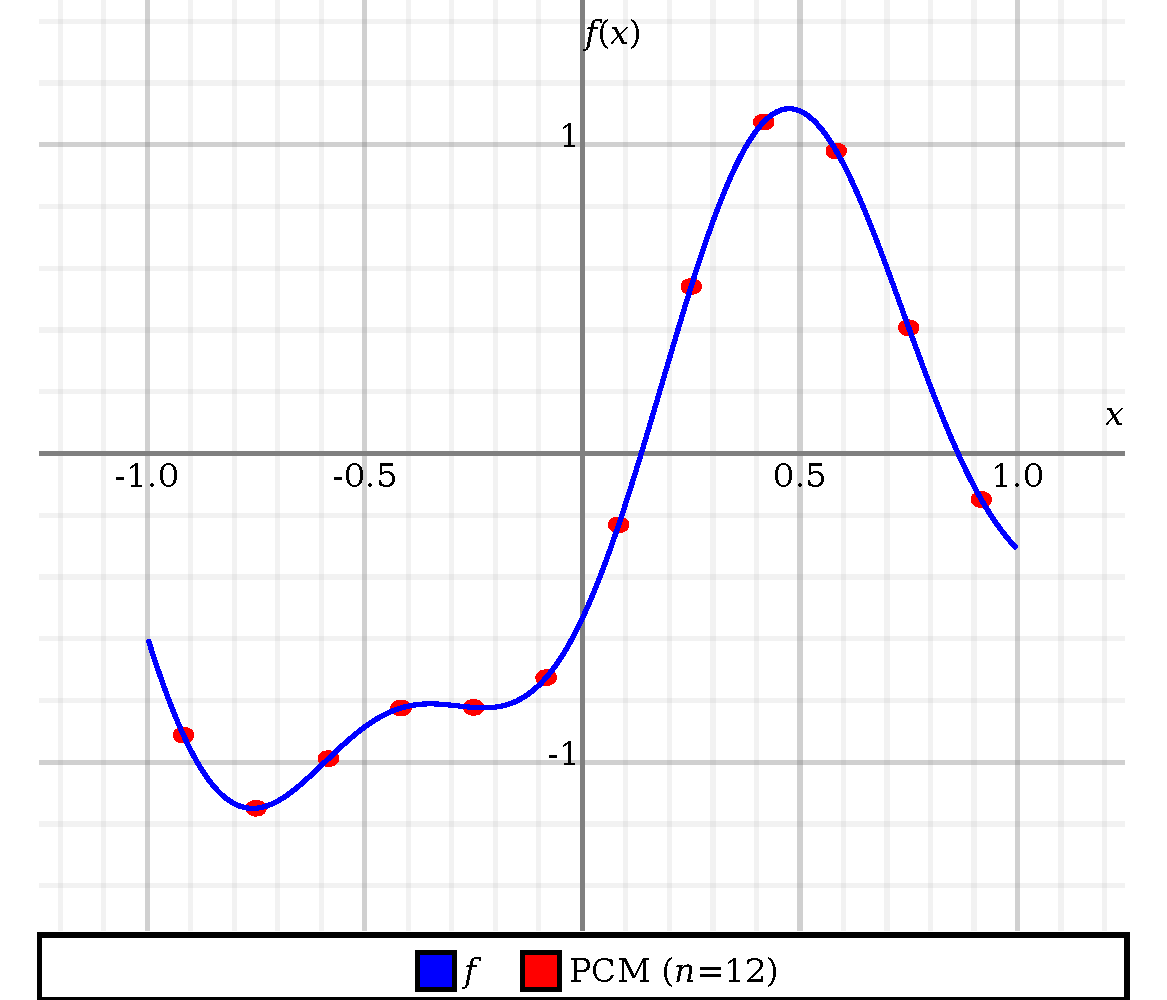
\includegraphics[width=\linewidth]{simple-PCM-example.pdf}
 \caption{Example of how a function $f:D^1\to\mathbb{R}$ is represented in PCM.}
 \label{haarDomDecompose}
\end{figure}
\begin{lstlisting}
newtype PCM_D¹ y = PCM_D¹ {
          getPCMSampling :: [y] }
\end{lstlisting}
where the \lstinline`y` values correspond to equally-spaced samples of the represented function, i.e.
\[
  \left[f(-1 + \tfrac2n\cdot i)\ \middle|\ i\leftarrow[\tfrac12\;..\;n-\tfrac12]\right].
\]
There is a body of theory, the \emph{Shannon-Nyquist formalism}, that makes PCM a quite solid method for representing a subspace of $\mathcal{L}^2$, the subspace of \emph{bandlimited} functions. We will not discuss this aspect here. 

The space of PCM-sampled functions is a vector space, and many applications make use of this fact all the time: array-languages like Matlab and NumPy implement addition, multiplication and more on arrays, and provided that all functions are sampled with the same resolution, this corresponds perfectly to the conceptually intended extensional addition of functions, i.e.
\begin{lstlisting}
h = PCM_D¹ $ zipWith (+)
    (getPCMSampling f) (getPCMSampling g)
\end{lstlisting}
\[
  \stackrel{\approx}{\Leftrightarrow} h(x) = f(x) + g(x).
\]
This does not hold up anymore if $f$ and $g$ are sampled at different resolution. Often, this is simply prevented altogether (made a runtime error or, somewhat better, type-error with indexed-length vector types).

In some applications this is not a problem: for example
\begin{itemize}
 \item In DSP, the input resolution is fixed by a physical ADC, and subsequent calculations (LTI filters etc.) simply leave it as-is or perhaps double the sampling. Nevertheless, it can be desirable to combine signals from different sources with different sampling rate, which then requires suitable resampling.
 \item Explicit integrators for hyperbolic PDEs iterate a re\-so\-lu\-tion-pre\-ser\-ving pro\-pa\-ga\-tor-trans\-for\-ma\-tion in\-vol\-ving the pointwise value of the old state and a numerical approximation (e.g. finite differences) of its spatial derivatives. This calculation will depend on the given resolution, but there is no need to precompute and store it in something like a matrix that would need to be valid for any of the possible resolutions: even if change of resolution should be required, the transformation can just be recomputed from scratch.
\end{itemize}
Many other applications, however, require coefficients to be stored before the required resolution is even known.
This is both necessary for implicit methods / inverse problems -- i.e. where there is no explitly programmed way to deduce the result from an input, but rather an input needs to be “guessed” that will match the desired output\footnote{
In practice, implicit methods use heuristics to choose a suitable resolution. A common approach is to just match the data count of the input to that of the intended output, which is reasonable enough since inversion is clearly dependent on some notion of isomorphism -- however, even an isomorphism does not necessarily preserve the highest, locally required resolution, but can “concentrate” data in given spots. This can again be taken into account with more heuristics to adaptively refine the mesh, or the extra detail can just be smoothed out (which can be useful to keep computation effort limited in nonlinear PDE solvers, however it is mathematically not really a correct solution then).
}, but also for calculations which simply require a stored-coefficient form for efficiency. Doing that in a general manner which would work regardless of what resolution turns out to be necessary in the end would amount to choosing an infinite resolution.

Experience with Haskell suggests that the problem of computing infinitely many coefficients should be possible with lazy evaluation, provided only finitely many of them actually need to be evaluated in the end.
However, a data structure like \lstinline`PCM_D¹` is not suitable for this, since adding new coefficients to the end of the list would change the meaning of the already calculated ones (they would be squeezed to the left of the domain).
What is required is some form of \emph{progressive} resolution.

\section{Multiscale resolution}\label{mulScaleResoIntro}
The main usefulness of spaces like $\mathcal{L}^2$ is that the infinite dimensionality can be managed easily if one only needs finite-width \emph{integrals} over the function, as these average out small-scale fluctuations.
To benefit from this, we must find a way to compute the integral without evaluating all the small-scale structure.
That is the idea behind multiscale or wavelet methods.
These are often derived as some orthonormal basis of $\mathcal{L}^2$, but we can also give a construction more from first principles.

To directly enable the $\mathcal{O}(1)$ evaluation of large-scale integrals, one might consider the following representation of $D^1\to \mathrm{y}$ functions:
\begin{lstlisting}
data PreIntg_D¹ y = PreIntg
   { offset :: y
   , lSubstructure :: PreIntg_D¹ y
   , rSubstructure :: PreIntg_D¹ y
   }
\end{lstlisting}
The idea is to decompose a function into a constant offset (proportional to the integral $\int_{D^1}\!\mathrm{d}x\:f(x)$) plus finer-grained fluctuations in each half of the domain, which are in turn recursively represented by the same type.
\[
  f_{(y_0,f_\mathrm{l},f_\mathrm{r})}(x)
      = y_0 + \begin{cases}
                 f_\mathrm{l}(x_\mathrm{l}) & \text{if $x$ on left}
              \\ f_\mathrm{r}(x_\mathrm{r}) & \text{if $x$ on right}
              \end{cases}
\]
The data structure \lstinline`PreIntg_D¹` defined above is a binary tree which has always infinite size.
This can be handled in a language with lazy evaluation like Haskell,
but only if all that is ever requested from the function are integrals over finite-extend subintervals.
Pointwise evaluation would recurse infinitely.

% Always and everywhere going to infinite resolution is overzealous for a function type.
Note also that it is not really a function from $D^1$ to $\mathrm{y}$ if it \emph{cannot} be evaluated at any individual point in $D^1$.
In practice, for any given real-world measured function, there will be only finitely many data points available at any given moment,
so at a sufficiently small scale one would eventually store \emph{only} the offset,
and assume that any smaller fluctuations are negligible.
% which is warranted to happen for a continuous function.
% one should be more precise, as to continuous functions here...

This eventual cutoff can be implemented by wrapping the substructure fields in \lstinline`Maybe`.
Here we define instead a specific constructor for the zero function (to improve the semantics of the generic \lstinline`Nothing` constructor).
We now obtain a conventional tree with finite depth.
Note that it can now also be strictly evaluated (here enforced by the exclamation marks).
\begin{lstlisting}
data PreIntg_D¹ y
      = PreIntgZero
      | PreIntg !y !(PreIntg_D¹ y)
                   !(PreIntg_D¹ y)
\end{lstlisting}
Pointwise function evaluation is then readily implemented recursively:
\begin{lstlisting}
evalPreIntg_D¹ :: AdditiveGroup y
     => PreIntg_D¹ y -> D¹ -> y
evalPreIntg_D¹ PreIntgZero _ = 0
evalPreIntg_D¹ (PreIntg y0 l r) x
   = y0 + if x < 0
           then evalPreIntg_D¹ l (2*x+1)
           else evalPreIntg_D¹ r (2*x-1)
\end{lstlisting}
Here, \lstinline`2*x+1` or \lstinline`2*x-1` “zoom in” onto the left or right half subinterval, depending on where \lstinline`x` lies.

\par
One downside of \lstinline`data PreIntg_D¹` is that it is redundant:
the offset already fixes what the integral over the complete function should be,
but there is nothing preventing the sub-interval functions from contributing their own part to the integral.
One solution is to use a type which represents functions having vanishing integrals.
This means there can be no global offset, instead the highest-level structure is the offset \emph{difference} between the domain halves.
This changes nothing about the data structure, just about its meaning:
\begin{lstlisting}
data HaarUnbiased y
     = HaarZero
     | HaarUnbiased !y !(HaarUnbiased y)
                       !(HaarUnbiased y)
\end{lstlisting}
Here, the \lstinline`y` value now represents the difference in offset between the left and right halves,
or, by our convention, the offset in the right half and, implicitly, the negated offset in the left half (which must be the same for the integral to vanish).
\begin{figure}
 \centering
 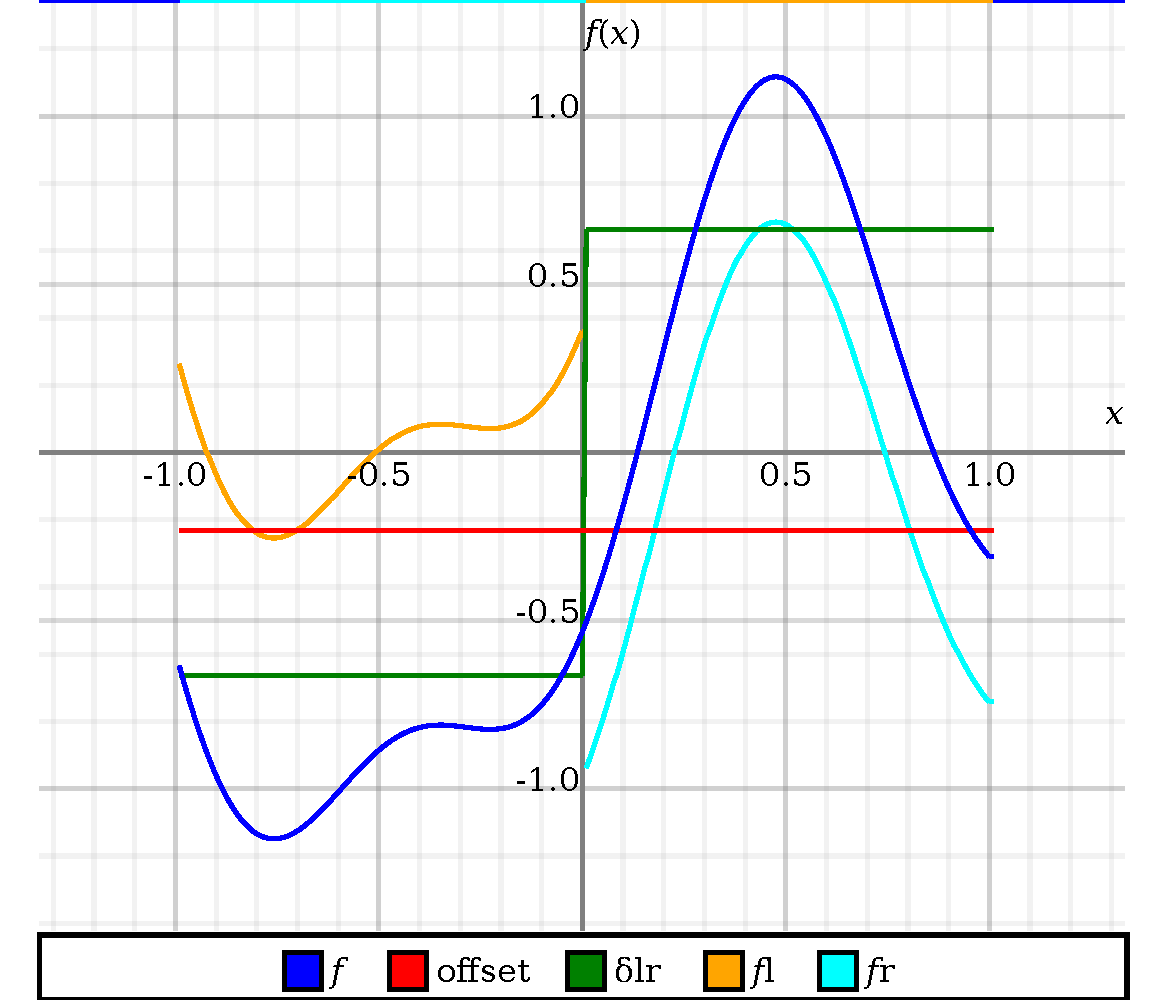
\includegraphics[width=\linewidth]{Haar-domDecompose.pdf}
 \caption{Example of how a function $f:D^1\to\mathbb{R}$ is decomposed into a constant offset, plus a step-function (Haar wavelet) for the offset-difference between left and right half, plus local fluctuations in each of the halves.}
 \label{haarDomDecompose}
\end{figure}
One can support functions with nonzero integral by simply adding an absolute offset with a wrapper-type at the top level:
\begin{lstlisting}
data Haar_D¹ y = Haar_D¹
    { global_offset :: !y
    , variation :: HaarUnbiased y }
\end{lstlisting}
The name “Haar” indicates that the basis functions of this data type (meaning those functions represented when exactly one of the fields of type ℝ in the \lstinline`HaarUnbiased ℝ` structure is 1, all other zero) are exactly the unnormalised Haar wavelets.

\section{Integration}
Whether using traditional orthonormal-basis methods, or the domain-decomposition approach introduced in \autoref{mulScaleResoIntro},
the numerical representations are obtained from integrating the function on an interval.
If the function is given as an analytic expression, it might be possible to calculate this integral exactly,
but this is typically impossible, and one resorts to numerical approximations.
All such approximations amount to some weighted average of the sample points:
\[
  \int_{D^1}\!\mathrm{d}x\:f(x) \approx \sum_i w_i\cdot f(x_i)
\]
with $x_i\in D^1$, $\sum_i w_i = 1$.
% For the choice of evaluation points and weights there are many different considerations to achieve good accuracy efficiently, this shall not be discussed here.
The choice of the evaluation points $x_i$ and weights $w_i$ are subject to considerations of efficiency and accuracy which we will not discuss here.

Crucially for our purposes, the calculation can be split up across the domain just like the recursive \lstinline`HaarUnbiased` data structure is:
\[
  \int_{D^1}\!\mathrm{d}x\:f(x)
    = \frac12\int_{D^1}\!\mathrm{d}x\:f(\tfrac{x-1}2)
    + \frac12\int_{D^1}\!\mathrm{d}x\:f(\tfrac{x+1}2)
\]
Observe that $\tfrac{x-1}2$ only evaluates on the left-, $\tfrac{x+1}2$ only on the right half of the domain.

This allows constructing the \lstinline`HaarUnbiased` tree in single pass with bottom-up propagation of the partial integrals, to obtain the offset estimates at each level without redundant computation.
The choice of numerical approximation only occurs at the smallest level;
the simplest possibility is to only evaluate it at a single point in the middle and give that full weight (rectangular method).
Thus the Haar representation can be obtained in $\mathcal{O}(n\cdot\log n)$ from a function on the interval:
\begin{lstlisting}
homsampleHaar_D¹ :: ( VectorSpace y
                    , Fractional (Scalar y) )
            => PowerOfTwo -> (D¹ -> y) -> Haar_D¹ y
homsampleHaar_D¹ (TwoToThe 0) f
   = Haar_D¹ (f 0) HaarZero
homsampleHaar_D¹ (TwoToThe i) f
   = case homsampleHaar_D¹ (TwoToThe $ i-1)
            <$> [ f . \x -> (x-1)/2
                , f . \x -> (x+1)/2 ] of
       [Haar_D¹ y0l sfl, Haar_D¹ y0r sfr]
        -> Haar_D¹ ((y0l+y0r)/2)
             $ HaarUnbiased ((y0r-y0l)/2) sfl sfr
\end{lstlisting}
This algorithm is in DSP called a \emph{fast wavelet transform}, which starts out with a PCM-sampled array instead of a function-to-be-sampled.
One advantage of our approach is that it is not necessary to select one global maximum resolution (here the \lstinline`PowerOfTwo` parameter); instead, a heuristic can be added that refines the resolution \emph{locally} until the function is satisfactorily approximated.
\begin{remark}
Similar adaptive resolution strategies often dramatically improve performance in real-world applications, such as physics/engineering simulations (finite elements or finite volumes methods, where they correspond to adaptive mesh refinement).
It is also the main principle behind image compression formats which use quantization on a wavelet expansion.
The reason is that images or solutions to nonliner differential equations are often quite smooth in most of the domain, but include sharp edges / transients / shocks confined to a much smaller area.
\end{remark}

\section{Square-integrable functions and beyond}
The \verb`Haar_D¹` structure as given in section \ref{mulScaleResoIntro}, with its strict spine and thus finite depth for every tree, can not represent every $D^1$ function. \footnote{Perhaps most strikingly, all these functions are \emph{dis}continuous. Like with PCM, this could be “fixed” through interpolation post-processing, but that does in neither case enable to exactly fit any function.}
It \emph{can} approximate arbitrarily well any $\mathcal{L}^2$ function (in the $\mathcal{L}^2$-norm sense). Namely, given a function \verb`f`, the sequence
\begin{lstlisting}
[homsampleHaar_D¹ (TwoToThe n) f | n<-[0..]]
\end{lstlisting}
converges to \verb`f`. This is much the same for a PCM representation: improving the resolution will allow it to match an $\mathcal{L}^2$ or continuous function ever better.

However, unlike with the PCM array representation, this progressive refinement of resolution does not change the top-level structure but only adds sub-branches at ever deeper levels in the trees. It is alluring to consider allowing the trees to have \emph{infinite} depth, which can readily be had in Haskell if only we drop the strictness annotations in the data structure. Would that then allow representing any $\mathcal{L}^2$ function \emph{exactly}?

It does not quite work this way, at least not practically:
\begin{itemize}
 \item \verb`evalPreIntg_D1` would recurse infinitely. So even if the infinite tree would theoretically represent the desired function, it would not be possible to evaluate it as such in finite time.
 \item \verb`homsampleHaar_D¹`, as it stands, would not be able to provide even the top-level node (i.e. the global integral), without first going into the local branches that are needed\footnote{
This could be overcome if we assume there is some other way of obtaining the target function's integral over a whole interval. However, \emph{if} that is possible, e.g. because the function is given by an analytical expression, then one does not really need to resort to a numerical representation!} to compute it.
\end{itemize}
Mathematically speaking, an infinite tree would correspond to an infinite sum over ever smaller Haar-wavelets. Infinite sums are possible to compute, provided they converge. What this means for practical computer applications is generally that the sum is \emph{not} evaluated completely, but only the finite partial sum that suffices to achieve the required precision (this also applies to other convergent sequences, e.g. Taylor expansion of an analytic function).
In other words, if the results need not be exact, then a finite cutoff of the converging-sum infinite tree is also sufficient, which is why we suggest keeping the \verb`Haar_D¹` structure strict/finite.

On the other hand, the coefficients in an infinite tree a in principle not constrained in a way that would require convergence. Thus they can also represent things that are not $D^1\to \mathbb{R}$ functions at all.

This is not as unreasonable as it may seem. In fact, particularly in physics, “limit functions” that are defined by a not-really-convergent sequence are quite commonly used, albeit often with lack of mathematical explanation. Best known, the “Dirac function”, informally defined as
\begin{align*}
  \delta &\colon \mathbb{R} \to “\mathbb{R}\cup\{\infty\}”
 \\
  \delta(x) &= \begin{cases} “\infty” & \text{if }x=0
                          \\ 0        & \text{otherwise} \end{cases}.
\end{align*}
The idea is that, the integral should come out as 1, and particularly for any other function $g$,
\[
  \int_\mathbb{R}\!\mathrm{d}x\: \delta(x)\cdot g(x) = g(0)
\]
should hold, allowing to rewrite pointwise evaluations as integrals vice versa. The integral over the product is also known as the $\mathcal{L}^2$ scalar product.

The above integral equation is quite tractable in a limit sense: consider a sequence of ever narrower and higher box-functions
\[
  \delta_{[n]}(x) = \begin{cases}
                           n   & \text{if $-\tfrac1n<x<\tfrac1n$}
                        \\ 0   & \text{else}
                       \end{cases}.
\]
Then
\[
  \int_\mathbb{R}\!\mathrm{d}x\: \delta_{[n]}(x)\cdot g(x)
    = n\cdot\int\limits_{-1/n}^{1/n}\mathrm{d}x\: g(x).
\]
If $g$ is continuous, then it will on the ever-smaller integration interval eventually behave like the constant $g_0$, and
\[
  n\cdot\int\limits_{-1/n}^{1/n}\mathrm{d}x\: g_0 = g_0 = g(0).
\]
This shows that the idea is sensible, but $\delta$ as a function is not: the sequence $(\delta_{[n]})_n$ does not converge, neither pointwise nor in the square-integral.

What does work about it really is just the \emph{contraction} / scalar product with $g$. 

By analogy, we propose that it would be useful to also consider infinite-depth trees, but not as a representation for functions on $D^1$ but just for contracting against such functions:
\begin{lstlisting}
data CoHaarUnbiased y
     = CoHaarZero
     | CoHaarUnbiased !y (HaarUnbiased y)
                         (HaarUnbiased y)
data CoHaar_D¹ y
     = CoHaar_D¹ !y (CoHaarUnbiased y)
\end{lstlisting}
Even though this is now non-strict, the following is guaranteed to terminate\footnote{%
This is in striking analogy with the Agda programming language, in which data types are strict by default but there is also \emph{co-data} (coinductive types) allowing for infinite streams.
} because \verb`Haar_D¹` has only finite depth and will thus eventually terminate the recursion:
\begin{lstlisting}
(<.>^) :: CoHaar_D¹ ℝ -> Haar_D¹ ℝ -> ℝ
CoHaar_D¹ q0 qFluct <.>^ Haar_D¹ f0 fFluct
    = q0 * f0 + qFluct~<.>^fFluct
 where CoHaarZero ~<.>^ _ = 0
       _ ~<.>^ HaarZero = 0
       CoHaarUnbiased δq ql qr
            ~<.>^ HaarUnbiased δf fl fr
          = δq * δf + ql~<.>^fl + qr~<.>^fr
\end{lstlisting}
This looks similar enough to a scalar product: corresponding entries in both of the tree structures are multiplied, and the results summed together -- like one would also do with the arrays of a PCM-representation. In both cases there are some constant factors missing to make it the actual $\mathcal{L}^2$ scalar product; we will ignore that here since anyways \verb`CoHaar_D¹ ℝ` has no interpretation as a type of functions on $D^1$ anymore.

Rather, it has an interpretation as a type of functions on \verb`Haar_D¹ ℝ`, i.e. (seeing \emph{those} as $D^1$-functions) higher order functions or \emph{functionals}, specifically linear functionals. (Linearity is important because these form themselves a vector space, the \emph{dual space}.)

The Dirac distribution is a very particular example of linear functional, that can indeed be implemented as a value of \verb`CoHaar_D¹ ℝ`. What it does -- evaluation at a single point -- is a special case of evaluation over a whole interval and averaging: essentially also what the elements of the $\delta_{[n]}$ sequence do, but because there is no explicit integral there is no need to scale up the height to infinity as the width is reduced.

\begin{lstlisting}
boxDistribution :: (D¹, D¹)  -- ^ Target interval
                -> ℝ         -- ^ Total weight
                -> Haar_D¹ DistributionSpace ℝ
boxDistribution (D¹ l, D¹ r) y
  | l > r      = boxDistribution (D¹ r, D¹ l) y
boxDistribution (D¹ (-1), D¹ 1) y
               = CoHaar_D¹ y zeroV
boxDistribution (D¹ l, D¹ r) y
  | l<0, r>0  -- intersecting both halves of domain
      = CoHaar_D¹ y $ CoHaarUnbiased (wr-wl) lstru rstru
  | l<0       -- target intersects only left half
      = CoHaar_D¹ y $ CoHaarUnbiased  (-wl)  lstru 0
  | otherwise -- target intersects only right half
      = CoHaar_D¹ y $ CoHaarUnbiased   wr    0   rstru
 where CoHaar_D¹ wl lstru = boxDistribution
                      (D¹ $ l*2 + 1, D¹ $ min 0 r*2 + 1)
                      (y * if r>0 then l/(l-r) else 1)
       CoHaar_D¹ wr rstru = boxDistribution
                      (D¹ $ max 0 l*2 - 1, D¹ $ r*2 - 1)
                      (y * if l<0 then r/(r-l) else 1)
\end{lstlisting}
The tree generated this way will in general have infinite depth in order to select the desired interval with any delimiters, i.e. this really requires the non-strict data structure.
However, the distribution will only narrow in on this selection provided that the function on which we evaluate has any structure at that level.
When the function is eventually constant, only the top-level coefficient is evaluated (as that corresponds to the integral, which is what is sought here).

Furthermore, \lstinline`boxDistribution` itself only builds up the infinitely fine resolution where it is actually required, i.e., at the \emph{boundaries} of the target interval:
on those subdivisions that are fully in the interval, again only to top-level coefficient of the function needs to be evaluated, whereas outside of the target the result will simply be zero.
Thus, the tree has only two long branches, and \lstinline`<.>^` has only a complexity of $\mathcal{O}(\log n)$ in the resolution of the function which the distribution is contracted against.
(Compare this with a PCM implementation, where a box distribution would need to contain $\mathcal{O}(n)$ nonzero entries, all of which would need to be evaluated.)

Finally, all of this works even if the target “interval” actually has zero width:
\begin{lstlisting}
dirac :: D¹ -> CoHaar_D¹ ℝ
dirac x0 = boxDistribution (x0,x0) 1
\end{lstlisting}

That implementation of the Dirac distribution does indeed evaluate functions of arbitrary resolution at one point. We have tested this with QuickCheck
As tested with QuickCheck,
\begin{lstlisting}
  testProperty "Dirac eval of Haar function"
   $ \f p -> dirac p<.>^f ~= evalHaarFunction f p
\end{lstlisting}
where the QuickCheck \lstinline`Arbitrary` instance generates arbitrarily deep tree structures, and picks any point on $D^1$ for evaluation.
\lstinline`~=` checks equality up to floating-point inaccuracy (in our test suite, the relative error  is set to $10^{-9}$).
Note that the behaviour, both of \verb`evalHaarFunction` and \verb`dirac` is strictly speaking undefined at the discontinuities created by the Haar representation, but the implementations shown here are in agreement. At any rate this seems safe as long as the \verb`Haar_D¹` function is an approximation of a continuous function, because then the jumps have only very small height.

\section{Tensor products and linear maps}

One of the most salient aspects about the dual space implementation is that it allows for a \emph{storable} implementation of arbitrary linear mappings.
\begin{lstlisting}
newtype LinearMap v w = LinearMap
           (TensorProduct (DualVector v) w)
\end{lstlisting}
The \lstinline`TensorProduct` for a parameterised type like \lstinline`Haar_D¹` and \lstinline`CoHaar_D¹` -- generally, for any functor in the category of vector spaces%
\footnote{They are in fact also functors in the \textbf{Hask} category, but we recommend keeping that instance a private implementation detail because fmapping a nonlinear function is not invariant of the choice of basis, i.e. it is not safe with respect to refactoring to another representations.
} -- is simply given by instantiating the parameter with the right factor space.
\begin{lstlisting}
type instance Scalar y ~ ℝ
   => TensorProduct (CoHaar_D¹ ℝ) w = CoHaar_D¹ w
\end{lstlisting}
So specifically, \lstinline`LinearMap (Haar_D¹ ℝ) (Haar_D¹ ℝ)` is represented by a distribution of functions, i.e. by of the type \lstinline`CoHaar_D¹ (Haar_D¹ ℝ)`.
This type is important because it would be the type of the identity linear mapping, which is required for \lstinline`Haar_D¹ ℝ` to be a member of an actual category and prerequisite for generalising several linear algebra algorithm from the finite-Euclidean case to infinite-dimensional spaces like \lstinline`Haar_D¹ ℝ`.
This is another reason why \lstinline`CoHaar_D¹` must be non-strict: the identity mapping must use an infinite tree, namely
\begin{lstlisting}
id :: LinearMap (Haar_D¹ ℝ) (Haar_D¹ ℝ)
id = LinearMap $ CoHaar_D¹
           (Haar_D¹ 1 zeroV)
           (fmap (\ δ -> Haar_D¹ 0 δ) idUnbiased)
 where idUnbiased :: TensorProduct (CoHaarUnbiased ℝ)
                                   (HaarUnbiased ℝ)
       idUnbiased = CoHaarUnbiased
        (CoHaar_D¹ 1 zeroV zeroV)
        (fmap (\l -> HaarUnbiased 0 l zeroV) idUnbiased)
        (fmap (\r -> HaarUnbiased 0 zeroV r) idUnbiased)
\end{lstlisting}

\section{Outlook}
Although the Haar-wavelet-expansion type presented in this paper provides a useful starting point for numerical calculations on infinite-dimensional spaces, the fact that the represented functions are inherently discontinuous step-functions limits its usefulness for actual numerical applications. The step functions certainly are not differentiable\footnote{%
They are differentiable \emph{almost} everywhere with derivative zero, but integrating that again would clearly not give back the original function but a constant!}.

Even for pointwise evaluation alone, the piecewise constant structure means that it is relatively inefficient at approximating continuous functions, namely, the discretisation error $\varepsilon = f_\text{exact} - f_\text{Haar}$ reduces proportionally to the step size $\delta$, i.e. anti-proportionally to the required tree size.
The adaptiveness of resolution can somewhat mitigate this (regions with small gradients have low $\varepsilon$ to begin with, so it is sufficient to focus on those with stronger gradient or even discontinuity), however this is limited unless the function really is constant on most of the domain.

By contrast, piecewise linear functions can scale $\varepsilon \propto \delta^2$, cubic ones $\varepsilon \propto \delta^4$ and so on. Thus it would be desirable to combine such a higher-order local model with the tree-based multiscale structure.
Comparison with wavelet theory suggests that this may not be as straightforward as it is to employ polynomial interpolation for a PCM sampling or for a finite elements model. Namely, the simplest piecewise-linear orthogonal wavelet is not a hat function by the rather complicated Strömberg wavelet.

However, our approach has the advantage that it does not actually rely on $\mathcal{L}^2$-orthogonality, but uses domain decomposition and direct value readoff for its sampling process. Therefore it is plausible that the “mother wavelet” can be kept much more basic.
In particular, a very simple way to construct a continuous function from a Haar-based one is through integration. Because the complete integral can always be evaluated in $\mathcal{O}(1)$, this would also still allow efficient random-access pointwise evaluation of the continuous function, unlike the integral of a PCM-sampled function (which would be $\mathcal{O}(n)$ for single-point evaluation).

Another important generalisation will be mul\-ti-di\-men\-sio\-nal domains. In fact, \lstinline`Haar_D¹` already supports those in a sense because a function vector space on a product domain is isomorphic to the tensor product of the function spaces on the factor domains, i.e. \lstinline`Haar_D¹ (Haar_D¹ ℝ)` represents functions on $D^1\times D^1$. 
However, this would largely circumvent the locality properties of the Haar expansions (since nearby points in y-direction would lie in completely different trees of the decomposition in x-direction). An efficient implementation would probably need to intersperse the di\-rec\-tion-split\-tings, to give a kind of $k\mathrm{d}$-tree structure in space an Morton Z order of the leaves.

In summary: we have presented a data structure that can express function types in a way that better represents the mathematical (functional-analysis) notion of such an infinite-dimensional space than the mainstream numerical expansions do.
It combines features of techniques from established numerical schemes (wavelets from multiscale analysis, tree backbones from Barnes-Hut style simulations, pa\-ra\-met\-ri\-ci\-ty/ten\-sor-pro\-duct from numerical linear algebra), and we expect that it can be extended to be of similar practical use while being more mathematically general and transparent.


%% Bibliography
%\bibliography{bibfile}



\end{document}
